\section{functions}

Let $f$ be a relation between two sets $A$ and $B$. We will use arrow notation,
so we will write $a\stackrel f\mapsto b$ if $(a,b)\in f$. We will say that $f$
is a function from $A$ to $B$ and write $f\colon A\to B$ if for every $a\in A$
there exists a unique $b\in B$ such that $a \stackrel f \mapsto b$. We might say
that $f$ is defined on $A$ (because for every point $a$ in $A$ there is an
outgoing arrow from $a$) and is unique (because such an arrow is unique).

Given $a\in A$, there exists a unique $b\in B$ such that $a\stackrel f \mapsto
b$: we will call this object $b$ either $fa$ or $f(a)$ \mymargin{$f(x)$} and say
that the function $f$ maps $a$ to $b$. Thus, we have
\[
 b=f(a) \iff a\stackrel f \mapsto b.
\]
The elements of the domain are often called \emph{points}, while the elements of
the codomain are called \emph{values}. The function $f$ will therefore have
value $f(a)$ at point $a$. The set of all functions $f\colon A\to B$ is usually
denoted by $B^A$ or $A\to B$. \mymargin{$B^A$} \index{$A^B$} \index{$A\to B$}
\index{power!sets}

\begin{figure}
  \mbox{}
  \hfill
  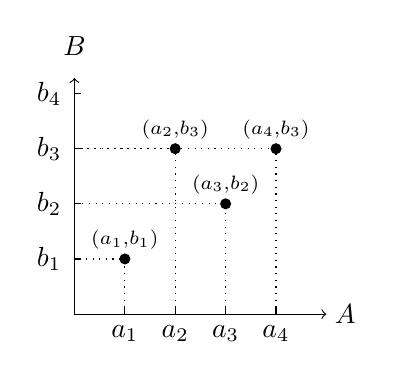
\begin{tikzpicture}[x=0.8cm]
  	\draw[->] (0,0) -- (4,0);
  	\draw[->] (0,0) -- (0,3.0);
  	\node at (4.3,0) {$A$};
  	\node at (0,3.4) {$B$};

      \draw (0.8,0) -- +(0,0.1) node [label=below:$a_1$]{};
      \draw (1.6,0) -- +(0,0.1) node [label=below:$a_2$]{};
      \draw (2.4,0) -- +(0,0.1) node [label=below:$a_3$]{};
      \draw (3.2,0) -- +(0,0.1) node [label=below:$a_4$]{};

      \draw (0,0.7) -- +(0.1,0) node [label=left:$b_1$]{};
      \draw (0,1.4) -- +(0.1,0) node [label=left:$b_2$]{};
      \draw (0,2.1) -- +(0.1,0) node [label=left:$b_3$]{};
      \draw (0,2.8) -- +(0.1,0) node [label=left:$b_4$]{};

  	\draw[dotted] (0.8,0) -- (0.8,0.7) -- (0,0.7);
  	\draw[dotted] (1.6,0) -- (1.6,2.1) -- (0,2.1);
  	\draw[dotted] (2.4,0) -- (2.4,1.4) -- (0,1.4);
  	\draw[dotted] (3.2,0) -- (3.2,2.1) -- (0,2.1);

  	\fill (0.8,0.7) circle (2pt) node[above] {$\scriptstyle (a_1,b_1)$};
  	\fill (1.6,2.1) circle (2pt) node[above] {$\scriptstyle (a_2,b_3)$};
  	\fill (2.4,1.4) circle (2pt) node[above] {$\scriptstyle (a_3,b_2)$};
  	\fill (3.2,2.1) circle (2pt) node[above] {$\scriptstyle (a_4,b_3)$};
  \end{tikzpicture}
\hfill
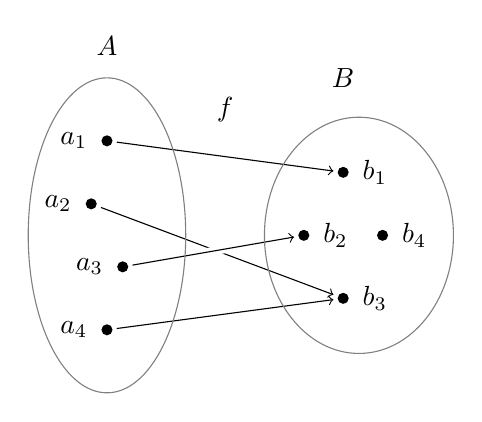
\begin{tikzpicture}[x=1cm,y=0.8cm]
\fill (1,4) circle (2pt) node (a1) [label=left:$a_1$]{};
\fill (0.8,3) circle (2pt) node (a2) [label=left:$a_2$]{};
\fill (1.2,2) circle (2pt) node (a3) [label=left:$a_3$]{};
\fill (1,1) circle (2pt) node (a4) [label=left:$a_4$]{};
\fill (4,3.5) circle (2pt) node (b1) [label=right:$b_1$] {};
\fill (3.5,2.5) circle (2pt) node (b2) [label=right:$b_2$] {};
\fill (4,1.5) circle (2pt) node (b3) [label=right:$b_3$] {};
\fill (4.5,2.5) circle (2pt) node (b4) [label=right:$b_4$] {};
\draw[->] (a1) edge (b1);
\draw[->] (a2) edge (b3);
\draw[line width=3pt,white] (a3) edge (b2);
\draw[->] (a3) edge (b2);
\draw[->] (a4) edge (b3);
\draw[draw=gray](1,2.5) ellipse (1cm and 2cm);
\draw[draw=gray](4.2,2.5) ellipse (1.2cm and 1.5cm);
\node at (1,5.5) {$A$};
\node at (4,5) {$B$};
\node at (2.5,4.5) {$f$};
\end{tikzpicture}
\hfill
\mbox{}
\caption[]{The function $f\colon A\to B$, $f=\{a_1\mapsto b_1,$ $a_2 \mapsto b_3,$ $a_3 \mapsto b_2,$ $a_4 \mapsto b_3\}$ defined on the set $A=\ENCLOSE{a_1, a_2, a_3, a_4}$ with values in the set $B=\ENCLOSE{b_1, b_2, b_3, b_4}$ represented via graph and Venn diagrams.}
\label{fig:funzione}
\end{figure}

The initial set $A$ is called the \emph{domain} \mymargin{domain} \index{domain}
of the function $f\colon A\to B$, while the target set $B$ is called the
\emph{codomain} \mymargin{codomain} \index{codomain}. The function $f$ thus
represents a way to uniquely assign to each element of the domain an element of
the codomain. From a computational perspective, we might say that $A$ is the set
of possible \emph{inputs} and $B$ is the set of possible \emph{outputs} of the
function $f$.

As we have defined it, a function is thus a set. In general, functions could be
defined in other ways or could be a primitive concept: thus, in the following
chapters, we will use functions without assuming that they are themselves sets.
For example, instead of writing $(a,b)\in f$, we will always write $f(a)=b$ or
$a\stackrel f \mapsto b$. It will still be very important to consider the set
that represents $f$, but this will be called the \emph{graph} \mymargin{graph}
\index{graph} of $f$, $G_f$, and can be defined in this way:
\[
  G_f = \ENCLOSE{(x,y)\in A \times B\colon f(x)=y}.
\]
In our construction, it turns out that $G_f = f$, but, as we have said, in
general, it is appropriate to distinguish the function from its graph. One of
the main topics of this course is the study of the graph of real functions, that
is, functions with domain and codomain in the set of real numbers.

\subsection{invertibility}

It often happens that a phenomenon can be mathematically modeled through a
function: it is known that a certain \emph{input} $a$ corresponds to an
\emph{output} $b=f(a)$. Very often, the problem to be solved is to determine the
correct \emph{input} $a$ to obtain the desired \emph{output} $b$. This problem
corresponds to \emph{inverting} the function $f$: given $b\in B$, determine
$x\in A$ such that $f(x) = b$.

A function $f\colon A \to B$ is said to be \emph{surjective}
\mymargin{surjective} \index{surjective} (or \emph{onto}) if for every $b\in B$,
there exists at least one $x\in A$ for which $f(x)=b$. This means that the
inversion problem has at least one solution, whatever $b\in B$ is. A function
$f\colon A \to B$ is said to be \emph{injective} \mymargin{injective}
\index{injective} if there do not exist two distinct points $a,a' \in A$, $a\neq
a'$, such that $f(a) = f(a')$. This means that the inversion problem $f(x)=b$
has at most one solution (the solution, if it exists, is unique). A function
$f\colon A \to B$ is said to be \emph{bijective} \mymargin{bijective}
\index{bijective} (or \emph{invertible}) \index{invertible}
\index{function!bijective} \index{invertible} \index{function!invertible}
\index{bijective} if it is both injective and surjective. This means that the
inversion problem $f(x)=b$ has a unique solution $x\in A$ for any $b\in B$. In
particular, if $f$ is invertible, for every $b\in B$, there exists a unique
$a\in A$ for which $f(a)=b$. If $f$ is an invertible function, then the inverse
relation $g$, that is, the relation such that $b\stackrel g \mapsto a$ when $a
\stackrel f \mapsto b$, turns out to be a function $g\colon B\to A$. Indeed, $g$
is defined on all of $B$ because $f$ is surjective, and $g$ is unique because
$f$ is injective. The characteristic properties of the \emph{inverse function}
\mymargin{inverse function} \index{function!inverse} $g$ are:
\begin{equation}\label{eq:572098}
  \forall a\in A\colon g(f(a)) = a, \qquad
  \forall b\in B\colon f(g(b)) = b.
\end{equation}
The function $g$ inverse to $f$ is usually denoted by the symbol $f^{-1}$.

If $f\colon A\to B$ is bijective, we will say that $A$ and $B$ are in
\emph{one-to-one correspondence} \mymargin{one-to-one correspondence}
\index{correspondence!one-to-one} through $f$. Indeed, $f$ is a \emph{unique}
correspondence from $A$ to $B$ (it uniquely maps each point of $A$ to a point of
$B$), and $f^{-1}$ is a unique correspondence from $B$ to $A$.

We now introduce some notations that will be convenient to use later. If
$f\colon A \to B$ is a function and if $C\subset A$, we define
\[
  f(C) 
  = \ENCLOSE{f(a)\colon a \in C} 
  = \ENCLOSE{b\in B\colon \exists a\in C\colon b=f(a)}.
\]
The set $f(C)\subset B$ is called the \emph{image} \mymargin{image set}
\index{image} \index{image!set} of $C$ (through $f$) and consists of all the
points obtained by applying $f$ to the elements of $C$. The image $f(A)$ of the
entire domain $A$ is called the image of $f$ and is sometimes denoted by the
symbol $\Im f$. Note that $f$ is surjective if and only if $f(A)=B$ (i.e., if
the image coincides with the codomain). For example, the function defined in
Figure~\ref{fig:funzione} has image $f(A) =
\ENCLOSE{f(a_1),f(a_2),f(a_3),f(a_4)} = \ENCLOSE{b_1, b_2, b_3}$.

Even if $f\colon A \to B$ is not injective, for every $C\subset B$, we can
define
\[
  f^{-1}(C) = \ENCLOSE{a\in A\colon f(a) \in C}.
\]
The set $f^{-1}(C)\subset A$ is called the \emph{preimage} or \emph{inverse
image} \mymargin{preimage} \index{preimage} \index{preimage!set} \index{inverse
image!set} \index{set!inverse image} of $C$ (through $f$) and consists of all
the points in $A$ that, when applying $f$, go into $C$. Note that if $b\in B$,
the set $f^{-1}(\ENCLOSE{b})$ is nothing other than the set of solutions to the
equation $f(x)=b$. As we have already seen, this set contains at least one
element if $f$ is surjective, contains at most one element if $f$ is injective,
and contains exactly one element $f^{-1}(\ENCLOSE{b}) = \ENCLOSE{f^{-1}(b)}$ if
$f$ is bijective. For example, if $f$ is the function defined in
Figure~\ref{fig:funzione}, we have $f^{-1}(\ENCLOSE{b_3,b_4}) =
f^{-1}(\ENCLOSE{b_3}) = \ENCLOSE{a_2,a_4}$, $f^{-1}(\ENCLOSE{b_4}) = \emptyset$.

The notation $f(C)$ just introduced is formally ambiguous because it might not
be clear whether $C$ is an element or a subset of the domain of $f$. In
practice, the context should make clear what is meant.

More generally, we will extend this abuse of notation not only to functions but
also to relations and operations. For example, if $A$ and $B$ are sets of
numbers, we might write $A\le B$ to mean that every element of $A$ is less than
or equal to every element of $B$, or $A+B$ to mean the set of all numbers
obtained by adding each number element of $A$ to each number element of $B$.

\begin{exercise}
    Let $f\colon A \to B$ be any function. Verify that if $C\subset A$ and
  $D\subset B$, then
  \[
    f^{-1}(f(C))\supset C,
    \qquad 
    f(f^{-1}(D)) \subset D. 
  \]
  
    What assumptions can we make about $f$ to have the equality $f(f^{-1}(C)) =
  C$? And to have $f^{-1}(f(D)) = D$?
\end{exercise}

Note that if $f\colon A \to B$ is a function and if $C\supset f(A)$, then
$f\colon A \to C$ as well, since the values of $f$ are elements of $C$. Thus,
the \emph{codomain} of a function can be extended or restricted with the care of
maintaining all the values of the image. In particular, $f\colon A \to f(A)$ is
certainly surjective.

For example, we will see that the function $\sin$ will be defined with domain
the set $\RR$ of real numbers but can have as codomain either $\RR$ itself or
only the interval $[-1,1]$ of numbers between $-1$ and $1$. It therefore makes
no sense to ask whether $\sin$ is surjective until I declare what the considered
codomain is: $\sin\colon \RR\to[-1,1]$ is surjective, while $\sin\colon
\RR\to\RR$ is not. Other texts consider the codomain part of the definition of
the function and therefore consider two functions with the same graph but
different codomain as different. It is a subtlety of little relevance.

To make a function injective, we must instead restrict the domain.

\begin{definition}[restriction]
  \label{def:restrizione}%
    If $f\colon A\to B$ is a function and $C\subset A$, we can \emph{restrict}
  the domain of $f$ to the set $C$. \mynote{The notation $f\llcorner C$ is not
  entirely standard, probably more common is the notation $f_{|C}$.} We obtain a
  new function $f\llcorner C$ that coincides with $f$ but is defined only on
  $C$: $f\llcorner C\colon C\to B$:
  \[
  f\llcorner C(x) = f(x)\qquad 
  \forall x \in C.
  \]
\end{definition}

\subsection{composite function}
\index{composition!of functions}%

If $f\colon A\to B$ and $g\colon B\to C$, then a point $a\in A$ is mapped by $f$
to a point $b\in B$, and in turn, the point $b$ is mapped by $g$ to a point $c
\in C$. The function that maps $a$ to $c$ is called the \emph{composite
function} \mymargin{composite function} \index{function!composite} and is
denoted by $g\circ f$ and can be defined as follows:
\[
g\circ f \colon A \to C, \qquad 
(g\circ f)(x) = g(f(x)).  
\]

If we have three functions $f\colon A\to B$, $g\colon B\to C$, and $h\colon C\to
D$, then it is easy to verify that:
\[
   h \circ (g\circ f) = (h\circ g) \circ f
\]
because for every $x\in A$, we have
\[
(h \circ (g\circ f)) (x) =
h(g(f(x))) = (h\circ g)(f(x)) = ((h\circ g) \circ f) (x).  
\]
This means that the composition operator $\circ$ satisfies the associative
property.

If $f\colon A\to B$ is bijective, then for every $x\in A$ and for every $y\in
B$, we have, thanks to~\eqref{eq:572098},
\[
  f^{-1} (f(x)) = x,
  \qquad f(f^{-1}(y)) = y.
\]
This means that 
\[
  f^{-1}\circ f = \id_A, 
  \qquad
  f\circ f^{-1} = \id_B
\] 
where $\id_X\colon X\to X$ is the \emph{identity} function \mymargin{identity}
\index{identity} \index{function!identity} that leaves every point of $X$ fixed:
\mymargin{$\id_X$} \index{$\id$}
\[
\id_X(x) = x \qquad \text{for every $x\in X$}.
\]

\begin{theorem}
If $f\colon A\to B$ and $g\colon B\to C$ are both invertible, then $g\circ
f\colon A\to C$ is also invertible, and we have
\begin{equation}\label{eq:inversa_composta}
  (g\circ f)^{-1} = f^{-1}\circ g^{-1}.
\end{equation}
\end{theorem}
\begin{proof}    
For every $c\in C$, there exists a unique $b\in B$ such that $g(b)=c$ and a
unique $a\in A$ such that $f(a)=b$. This $a$ is the only point for which
$g(f(a))=c$, and this shows that $g\circ f$ is bijective. Moreover,
$a=f^{-1}(b)$ and $b=g^{-1}(c)$, so $(g\circ f)^{-1}(c) = a =
f^{-1}(g^{-1}(c))$, from which we obtain \eqref{eq:inversa_composta}.
\end{proof}

\begin{exercise}
    Verify that the composition of injective functions is injective and the
  composition of surjective functions is surjective.
\end{exercise}

\begin{theorem}[Cantor-Bernstein]%
  \label{th:cantor_bernstein}%
  \index{theorem!Cantor-Bernstein}%
  \index{Cantor-Bernstein!theorem of}%
    If there exists $f\colon A \to B$ injective and $g\colon B\to A$ injective,
  then there exists $h \colon A \to B$ bijective.
\end{theorem}
%
\begin{figure}
  \centering
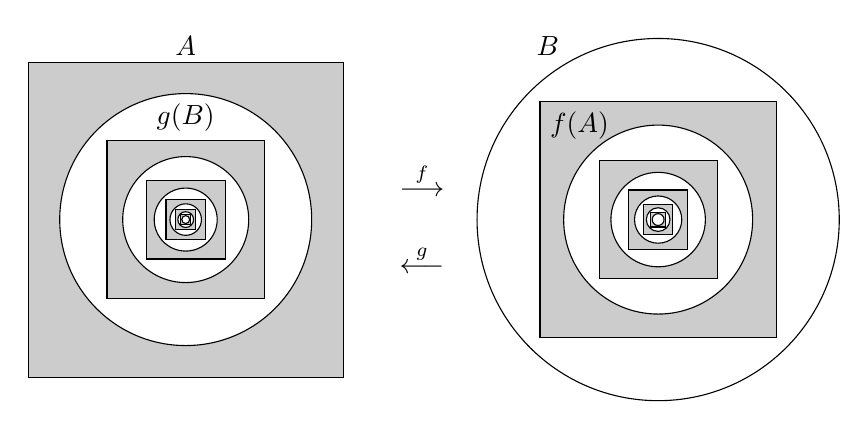
\begin{tikzpicture}
    \foreach \x in {1,0.5,0.25,0.25*0.5,0.25*0.25,0.25*0.25*0.5} {
      \path[draw,fill=black!20] (2*\x,2*\x)--(-2*\x,2*\x)--(-2*\x,-2*\x)--(2*\x,-2*\x)--cycle;
      \draw[fill=white] (0,0) circle (1.6*\x);
    };
    \node at (0,2.2) {$A$};
%    \node at (-1.3,1.65) {$A\setminus g(B)$};
    \node at (0,1.3) {$g(B)$};

    \node at (3,0.5) {$\stackrel f \longrightarrow$};
    \node at (3,-0.5) {$\stackrel g \longleftarrow$};

    \draw[fill=white] (6,0) circle (2.3);
    \foreach \x in {0.75,0.5*0.75,0.25*0.75,0.5*0.25*0.75,0.25*0.25*0.75} {
      \path[draw,fill=black!20] (6 + 2*\x, 2*\x)--(6 - 2*\x, 2*\x)--(6 - 2*\x,-2*\x)--(6 + 2*\x,-2*\x)--cycle;
      \draw[fill=white] (6,0) circle (1.6*\x);
      };
    \node at (4.6,2.2) {$B$};
%    \node at (6,1.9) {$B\setminus f(A)$};
    \node at (5,1.2) {$f(A)$};
\end{tikzpicture}

\caption{
    In the proof of the Cantor-Bernstein theorem, $A$ is represented by a square
  and $B$ by a circle contained in $A$. The image of $A$ in $B$ is represented
  by a square contained in $B$, and so on. The shaded part in set $A$ goes to
  the shaded part in set $B$ through $f$, while the white part goes to the white
  part.
  }
  \label{fig:omotetia}
\end{figure}
%
\begin{proof}
\emph{Step 1:} show that without loss of generality, we can assume $B\subset A$ and $g(x)=x$. Indeed, note that in general $g\colon B\to g(B)$ is a bijection and thus has an inverse function $g^{-1}\colon g(B)\to B$. If we consider $\tilde f = g^{-1}\circ f$, we then have an injective function $\tilde f\colon A \to g(B)\subset A$. If the theorem is true in this case (we will see in the next step), we will have a bijection $\phi\colon A\to g(B)$. Composing $\phi$ with $g^{-1}$ will yield a bijection between $A$ and $B$.

\emph{Step 2:} Suppose that $B\subset A$ and that $f\colon A \to B$ is injective. Intuitively, the idea is to define the set
\[
 D = (A\setminus B)  
 \cup f(A\setminus B) 
 \cup f(f(A\setminus B)) 
 \cup \dots
\]
and to define the bijection $\phi \colon A \to B$ using $f$ on the set $D$ and
leaving the rest fixed.

To do this rigorously, consider the family of sets $\F = \{X \subset A \colon X
\supset A \setminus B, f(X) \subset X\}$ and define $D = \bigcap \F$. Note that
$A \in \F$, so $\F\neq \emptyset$. We have essentially defined $D$ as the
smallest subset of $A$ that is mapped into itself by $f$.

It is easy to verify that $f(D) \subset D$; indeed, given $x\in D$, for every
$X\in \F$, it must be $x\in X$, but then $f(x) \in X$ (by the definition of
$\F$), thus $f(x) \in D$. Similarly, it is shown that $D\supset A\setminus B$,
and thus we conclude that $D\in \F$.

Now verify that $f(D)=D\cap B$. On one hand, if $x\in D$, then $f(x) \in
f(D)\subset D$ and $f(x)\subset f(A)\subset B$, hence $f(x) \in D\cap B$. On the
other hand, if $y\in D \cap B$ and it were not $y \in f(D)$, then we could
consider the set $X=D\setminus\{y\}$ and observe that $X\in \F$. Indeed, firstly
$X \supset A \setminus B$ because $D$ has this property and $y \in B$. Moreover,
given any $x \in X$, since $X\subset D$, then $f(x) \in f(D)$ and, by
hypothesis, $y\not \in f(D)$, hence $f(x)\neq y$, so $f(x) \in X$. Thus $X\in
\F$, but then it should be $D\subset X$, while by construction, we have $y\in D$
but not in $X$.

% Having seen that $f(D)=D\cap B$, we can easily observe that $f(A\setminus D) \subset A \setminus D$. Indeed, $f(A\setminus D)\subset f(A)=B$, and therefore $f(A\setminus D)\cap D \subset D \cap B = f(D)$, but since $f$ is injective, it must be $f(A\setminus D) \cap f(D)=\emptyset$.

We can then define $\phi \colon A \to B$ as
\[
\phi(x) =
\begin{cases}
   f(x) & \text{if $x\in D$}, \\
   x & \text{otherwise.}
\end{cases}
\]
Clearly, $\phi$ is injective because $f$ is injective and maps $D$ into $D\cap B
\subset D$, while the identity is injective and maps $A\setminus D$ into
$A\setminus D$.

To prove that $\phi$ is surjective, consider any $y \in B$. If $y\not \in D$,
then $\phi(y)=y$. If instead $y\in D$, being $y\in D\cap B = f(D)$, there will
exist $x\in D$ such that $\phi(x) = f(x) = y$.
\end{proof}